\chapter{Gravity, Mass, and the Idea of a Black Hole}
\label{ch:f1}

\noindent\emph{This first part of the report assumes no physics background at
all. It explains, in ordinary language, every idea the technical chapters
build on. If you are comfortable with general relativity, skip directly to
Part~II.}

\section{Throwing things upward}

Throw a ball into the air and it comes back. Throw it harder and it climbs
higher before it comes back. This everyday fact hides a precise question:
\emph{is there a throwing speed so great that the ball never comes back at
all?}

There is. For every planet or star there is a special speed, the
\emph{escape velocity}, at which a thrown object just barely coasts away
forever, slowing all the while but never quite stopping. From the surface of
the Earth it is about 11~kilometres per second — thirty times the speed of
sound. From the surface of the Sun it is about 620 kilometres per second.
The rule of thumb is simple: the more mass squeezed below you, and the
closer you stand to it, the faster you must go to leave.

\begin{worked}{How fast must you throw?}
The escape velocity has a one-line recipe. A thrown object escapes if
its energy of motion, $\tfrac12 v^2$ for every kilogram of it, at least
matches the energy needed to climb out of the gravity well, $Gm/r$ per
kilogram — where $m$ is the planet's mass, $r$ its radius, and $G$ is
Newton's gravitational constant, $6.67\times10^{-11}$ in SI units.
Setting the two equal and solving for $v$:
\[
v_{\rm esc}=\sqrt{\frac{2Gm}{r}}.
\]
For the Earth, $m = 5.97\times10^{24}$~kg and $r = 6\,371$~km, so
$2Gm = 7.97\times10^{14}$~m$^3$/s$^2$; dividing by
$r = 6.371\times10^{6}$~m gives $1.25\times10^{8}$~m$^2$/s$^2$, and the
square root is $11\,200$~m/s — the 11~km/s quoted above. Notice that
nothing in the formula cares what the ball is made of: only total mass
and radius enter. That indifference is the loophole a black hole
exploits.
\end{worked}

That second part — \emph{the closer you stand} — is the key to everything
in this report. Squeeze the same mass into a smaller ball and its surface
moves closer to the centre, so the escape velocity from that surface goes
up, even though the total mass never changed. Squeeze the Sun to a radius of
three kilometres and the escape velocity at its surface would reach the
fastest speed there is: the speed of light, about
300\,000~kilometres per second.

\section{The point of no return}

Light's speed is not just fast; physics as we understand it (and as
Chapter~\ref{ch:f2} sketches) says nothing can move faster. So an object
compressed within that critical size has a startling property: at some
radius, not even light travels fast enough to escape. Whatever falls inside
can send no signal out. The sphere where escape would require exactly the
speed of light is called the \emph{event horizon}: an ``event'' happening
inside it can never be seen from outside, even in principle.

An object like this is a \emph{black hole} — black because no light leaves
it, and a hole because things can fall in but not climb out. The critical
radius is named the \emph{Schwarzschild radius} after Karl Schwarzschild,
who solved Einstein's equations for a single round mass within weeks of
their publication in 1915. The Schwarzschild radius grows in direct
proportion to the mass: double the mass and the horizon doubles in size.
For the Earth it is about nine millimetres — the Earth would have to be
crushed to the size of a marble. For the Sun, about three kilometres. For
the black hole at the centre of our Galaxy, which weighs about 4.3 million
Suns, it is around 13 million kilometres — some eighteen times the radius
of the Sun, yet still tiny on galactic scales.

Two cautions about the picture this conjures. First, the horizon is not a
surface you could touch: nothing is \emph{there}. It is a boundary drawn in
empty space, the line on the map beyond which no path leads back out. A
falling astronaut would notice nothing special while crossing it. Second,
the mass is not spread throughout the dark sphere. As far as the theory can
say, everything that fell in is concentrated at the centre in a region
where the equations lose their meaning — the \emph{singularity}. The
singularity is a statement of ignorance rather than a physical prediction:
it marks where the current theory of gravity stops being trustworthy.
Fortunately, for everything in this report only the \emph{outside} of the
horizon matters, and there the theory is precise and testable.

\begin{worked}{The size of \sgra{}'s horizon}
Ask the escape-velocity recipe a pointed question: at what radius does
$v_{\rm esc}$ reach the speed of light? Set $v_{\rm esc}=c$ and solve
for the radius:
\[
R_S=\frac{2Gm}{c^2}.
\]
For \sgra{}, $m = 4.297$ million solar masses
$= 4.297\times10^{6}\times1.989\times10^{30}~{\rm kg}
= 8.55\times10^{36}$~kg. Then $2Gm = 1.14\times10^{27}$ in SI units,
and dividing by $c^2 = 9.0\times10^{16}$~m$^2$/s$^2$ gives
\[
R_S = 1.27\times10^{10}~{\rm m} \approx 12.7\ \hbox{million km},
\]
about eighteen Sun-radii, as quoted in the text; light itself would
need 42 seconds to cross that distance. One honest caution: we used
Newton's energy formula in a regime where Newton's theory fails. By a
happy algebraic coincidence the fully relativistic calculation
(Chapter~\ref{ch:kerr}) returns \emph{exactly} the same $R_S$ — which
is why this little derivation, essentially the one John Michell wrote
down in 1784, is worth showing at all.
\end{worked}

\section{Falling in: the gentle giant surprise}

One more everyday idea unlocks a real result. Stand on the Earth and
your feet are pulled slightly harder than your head — they are closer
to the centre. Near a compact mass this difference, the \emph{tidal}
force, can become violent: fall feet-first toward a small black hole
and the pull on your feet so exceeds the pull on your head that you
would be stretched like taffy (astrophysicists genuinely say
\emph{spaghettification}).

Here is the surprise: the bigger the black hole, the \emph{gentler}
its horizon. The tidal stretch across a falling body depends on the
mass divided by the \emph{cube} of the distance, and since the horizon
radius grows in proportion to the mass, the stretch \emph{at the
horizon} falls off as one over the mass squared. Crossing the horizon
of a 10-solar-mass black hole, the difference in pull across a
two-metre astronaut is about $2\times10^{8}$~m/s$^2$ — twenty million
times Earth's gravity, lethal long before arrival. Crossing the
horizon of \sgra{}, four hundred thousand times heavier, the same
difference is about one \emph{millimetre} per second squared — less
than the tug your feet feel from standing on a kerb. An astronaut
would drift across \sgra's point of no return without a twinge,
noticing nothing at all; the drama is reserved for much deeper in.
This is why nothing dramatic marks the horizon in the renders of this
report: general relativity says, correctly, that locally there is
nothing there (the caution of the previous section made precise).

\section{Sagittarius A*, our own giant}

Point a telescope at the constellation Sagittarius and you look toward the
centre of the Milky Way, 8\,277 parsecs away (a \emph{parsec} is about 3.26
light-years; the light arriving tonight left before the last ice age
peaked). At the exact dynamical centre sits a compact radio source named
\sgra{} (``Sagittarius A star''). Around it, stars swarm at extraordinary
speeds — a few pass their closest approach at several thousand kilometres
\emph{per second}, about a hundred times faster than the Earth orbits the
Sun. Something enormously heavy and enormously compact must be holding
them: the measured mass is $4.297\pm0.012$ million solar masses, packed
into a region smaller than the orbit of Mercury. No cluster of dim stars,
no exotic gas cloud survives scrutiny as an alternative; a supermassive
black hole is the only explanation standing
(Chapter~\ref{ch:intro} gives the observational history).

\sgra{} is the star of this report for a practical reason: it is the
\emph{nearest} supermassive black hole, and the only one where two entirely
different kinds of measurement meet. We can follow individual stars looping
around it year by year (Chapters~\ref{ch:f5}, \ref{ch:sstar},
\ref{ch:fitting}), and we can photograph the glowing ring of light bent
around its horizon (Chapters~\ref{ch:f3}, \ref{ch:shadow}). This report
describes a simulator built from first principles that reproduces both
kinds of measurement from the same underlying equations.

\section{A sense of scale}

The numbers in this subject span so many powers of ten that it is worth
pausing to place them on one line (Fig.~\ref{fig:dgscales}).

\begin{figure}
\centering
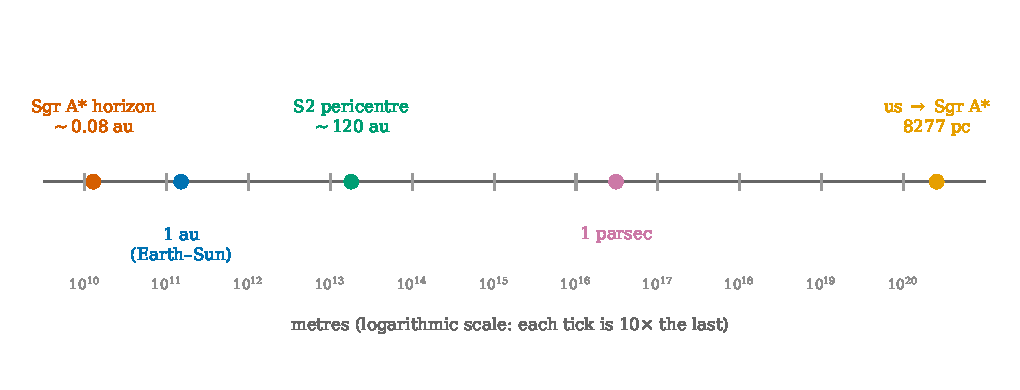
\includegraphics[width=\textwidth]{figures/dg_scales.pdf}
\caption{The scales of the problem on a single logarithmic line, from the
\sgra{} horizon to its distance from us. Each tick is ten times the
previous one: the distance to \sgra{} is about twenty billion times the
size of its horizon — comparable to viewing a coin at the distance of the
Moon.}
\label{fig:dgscales}
\end{figure}

Astronomers measure distances within a planetary system in
\emph{astronomical units} (au): one au is the Earth–Sun distance, about 150
million kilometres. The horizon of \sgra{} spans about a sixth of an
au. The star S2, the most important character of Part~III, dives to about
120~au from the black hole — about three times the distance of Pluto from
the Sun — which sounds close until you recall that this is still about
1\,500 horizon radii out.

For things on the sky, astronomers use angles. A degree is what your little
finger covers at arm's length; an \emph{arcsecond} is 1/3600 of a degree,
roughly a coin seen from four kilometres away; and the measurements in this
report are made in \emph{milliarcseconds} (a thousandth of an arcsecond)
and \emph{microarcseconds} ($\muas$, a millionth). The photon ring of
\sgra{} spans about 52~$\muas$ — the apparent size of a doughnut on the
Moon. That such an angle is measurable at all, by linking radio telescopes
across the whole Earth into one instrument, is among the technical wonders
of modern astronomy.

One more unit will keep appearing: the \emph{gravitational radius}, written
$M$ in this report. It is the natural yardstick of a black hole — half the
Schwarzschild radius — and it lets us describe any black hole, whatever
its mass, with the same numbers. ``The disk's inner edge sits at $6\,M$''
is true of a stellar black hole and of \sgra{} alike; only the metre-stick
changes. Chapter~\ref{ch:f6} says more about this trick of working in
natural units.

\begin{termsbox}
\item[Escape velocity] The launch speed at which an object barely coasts
away from a mass forever.
\item[Event horizon] The boundary around a black hole from inside which
nothing, not even light, can escape. Not a material surface.
\item[Schwarzschild radius] The size of the event horizon of a
non-spinning mass; proportional to the mass.
\item[Singularity] The central region where the known equations of gravity
break down; hidden inside the horizon.
\item[\sgra{}] The 4.3-million-solar-mass black hole at the centre of the
Milky Way, 8\,277 parsecs away.
\item[au, parsec, milli-/microarcsecond] Units for distances and sky
angles; see Fig.~\ref{fig:dgscales}.
\item[Gravitational radius ($M$)] The natural length unit of a black hole;
the horizon of a non-spinning hole sits at $2\,M$.
\end{termsbox}

\noindent$\rightarrow$ \emph{Full treatment: the observational case for
\sgra{} in Chapter~\ref{ch:intro}; the exact horizon formulas in
Chapter~\ref{ch:kerr}.}
